%\newcommand{\F}{\mathbb{F}}
%\newcommand{\G}{\mathbb{G}}
\newcommand{\Cdel}{\ensuremath{c_{del}}}
\newcommand{\Cins}{\ensuremath{c_{ins}}}
\newcommand{\Cupd}{\ensuremath{c_{upd}}}
\renewcommand{\O}{\ensuremath{\mathcal{O}}}

\chapter{Tree-edit-distance algoritmus}

Jadro aplikacie lezi v pouziti tree-edit-distance (TED) algoritmu,
vdaka ktoremu dostaneme mapovanie medzi 2 RNA stromami. Mapovanie nam ukaze
spolocne casti oboch RNA stromov. TED algoritmus je obdoba Levenstheinoveho
string-edit-distance algoritmu. Problem u retazcov je specialnym pripadom
TED-u, kedy stromy zdegenerovali na cesty (spojovy zoznam).

\section{Hlavna myslienka TED-u}

Zaklad TED algoritmu je v rekurzivnom vzorci \ref{eq:ted} z \citet{DMRW} a \citet{RTED}. Vzdialenost medzi
lesmi F a G, $\delta(F, G)$ je definovana ako minimalny pocet editacnych operacii,
ktore z F urobia G. Pouzivame standardne editacne operacie - delete, insert, update.

\begin{figure}[H]
\centering
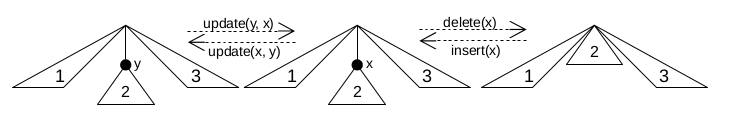
\includegraphics[width=140mm, height=30mm]{../img/TED_operations.png}
\caption{Ukazky TED operacii}
\label{obr:TED_operations}
\end{figure}

Delete, zmazanie vrcholu, znamena pripojit k predkovi vsetkych jeho potomkov so
zachovanim poradia medzi nimi. Insert, vlozenie vrcholu, je opacna operacia k
delete, co znamena, ze vkladame vrchol medzi rodica nejakych jeho, po sebe
nasledujucich potomkov. Update iba zmeni hodnotu vo vrchole stromu.

\section{Znacenie}

V tejto kapitole sa budeme riadit znacenim \citet{RTED}. Teda, pouzivame definiciu
stromu a lesa z \ref{def:strom}. Ak $F$ je les (strom), $N_F$ oznacuje mnozinu jeho vrcholov a $E_F$
mnozinu jeho hran. Plati dalej ze $E_F \subseteq N_F \times N_F$. $\emptyset$ oznacuje
prazdny strom, resp. prazdny les. Podles lesa $F$ je graf $\tilde{F}$ s vrcholmi
$N_{\tilde{F}} \subseteq N_F$ a hranami $E_{\tilde{F}} \subseteq E_F \cap N_{\tilde{F}} \times N_{\tilde{F}}$.
Obdobne to plati aj pre podstrom stromu $T$.
$F_{v}$ oznacuje podstrom $F$ zakoreneny vo $v$, t.j. v strome ostavaju iba potomkovia $v$.
$F - v$ budeme znacit les, ktory dostaneme zmazanim vrcholu $v$ z $F$, spolu so vsetkymi hranami
zasahujucimi do $v$. Podobne $F - F_{v}$ budeme znacit les, ktory dostaneme zmazanim podstromu
$F_{v}$ z $F$.

\begin{definice}[Editacna vzdialenost]
	Nech F a G su dva lesy. Editacna vzdialenost, tree-edit-distance - $\delta(F, G)$,
	medzi F a G je rovna minimalnej cene, za ktoru les F transformujeme na G.
\end{definice}

Vo vzorci \ref{eq:ted} pocitame editacnu vzdialenost $\delta(F, G)$,
\Cdel, \Cins a \Cupd su ceny zmazania, vlozenia a editacie vrcholu v strome
a $r_{F}$ a $r_{G}$ su korene, bud obidva najpravejsie alebo najlavejsie (tzn. vyberieme
najpravejsi/najlavejsi strom lesa a jeho koren).

\begin{figure}[H]\label{eq:ted}
\begin{subequations}
\begin{align}
	\begin{split}
	\delta(\emptyset, \emptyset) &=
		0
		\\
	\delta(F, \emptyset) &=
		\delta(F - r_{F}, \emptyset) + \Cdel(r_{F})
		\\
	\delta(\emptyset, G) &=
		\delta(\emptyset, G - r_{G}) + \Cins(r_{G})
	\end{split}
	\\[1ex]
	\delta(F, G) &=
		\begin{cases}
			\delta(F - r_{F}, G) + \Cdel(r_{F}) \\
			\delta(F, G - r_{G}) + \Cins(r_{G}) \\
			\delta(F - F_{r_{F}}, G - G_{r_{G}}) + \\
				\quad \delta(F_{r_{F}} - r_{F}, G_{r_{G}} - r_{G}) + \Cupd(r_{F}, r_{G})
		\end{cases}
\end{align}
\end{subequations}
\caption{Rekurzivny vzorec pre vypocet tree-edit-distance}
\end{figure}

\section{Algoritmy dynamickeho programovania}

Kazdy krok rekurzie \ref{eq:ted} je vypocitana v konstantnom case z inych podproblemov,
takze doba behu algoritmu zavisi na pocte podproblemov, ktore sa budu pocitat.
Rekurzia medzi lesmi $F$ a $G$ vedie k casovej zlozitosti $\O(n^2 \cdot m^2)$
a priestorovej zlozitosti $\O(n \cdot m)$ kde $n = N_F$ a $m = N_G$.

\begin{definice}[Dekompozicna strategia]
	TODO
	% TODO
\end{definice}

Zvysovaniu efektivity algoritmu sa venuju \citet{ZHANGSHASHA}, \citet{DMRW} a \citet{RTED}.
Posledny menovany vyuziva 

\begin{definice}
	Celkova dekompozicia lesa (full decomposition) $F$, $\mathcal{A}(F)$ je mnozina
	vsetkych podlesov F, ktore dostaneme rekurzivnym odstranenim najlavejsieho
	alebo najpravejsieho korenoveho vrcholu - $r_{R}(F)$ a $r_{L}(F)$ z $F$
	a nasledne aj vsetkych jeho podlesov.
	\begin{align*}
		\quad{} \mathcal{A}(\emptyset) &= \emptyset
		\\
		\quad{} \mathcal{A}(F) &= {F} \cup \mathcal{A}(F - r_{L}(F)) \cup \mathcal{A}(F - r_{R}(F))
	\end{align*}
\end{definice}



